	\begin{figure}[!h]
		\centering
 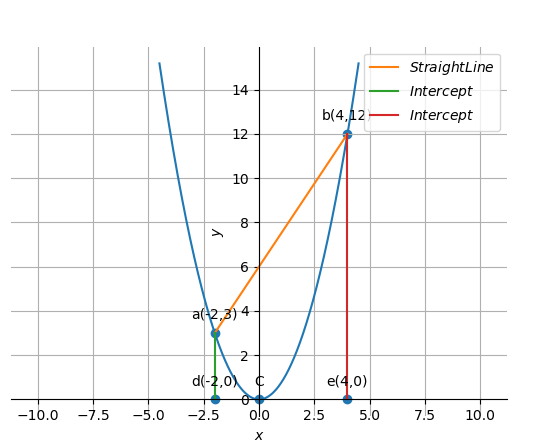
\includegraphics[width=\columnwidth]{chapters/12/8/3/7/figs/conic.png}
		\caption{}
		\label{fig:12/8/3/7}
  	\end{figure}
The parameters of the given conic are
\begin{align}
\vec{V}=\myvec{
3 & 0\\
0 & 0
},
\vec{u}=\myvec{0\\-2},
f=0.
\end{align} 
For the line, the parameters are
\begin{align}
\vec{h} = \myvec{
-2\\
3
},
\vec{m} = \myvec{2 \\ 3}
\end{align}
yielding
\begin{align}
    \kappa=-2.5,2.7
\end{align}
upon substitution in \eqref{eq:tangent_roots}
resulting in the points of intersection
\begin{align}
    \vec{A}=\myvec{
-2\\
3
    },
    \vec{B}=\myvec{
4\\
12
    }.
\end{align}
From 
		\figref{fig:12/8/3/7},
the desired area is 
\begin{align}
\int_{-2}^{4} \frac{3x+12}{2} \,dx
-\int_{-2}^{4}\frac{3x^2}{4} \,dx 
= 27 
\end{align}
